\documentclass[../Main.tex]{subfiles}
\begin{document}
  \chapter{2017-2018学年微积分（一）（下）期中考试}

  \section{基本计算题(每小题 6 分，共 60 分)}
  \begin{enumerate}
    \item 设直线$l$过点$M_{0}(1,2,0)$，且平行于平面$\pi:x-2y+z-4=0$，又与直线$l_{1}
      :\frac{x-2}{1}=\frac{y-1}{2}=\frac{z-2}{1}$相交，求此直线的方程.
      \vspace{10em}

    \item 求曲线$\begin{cases}
        x^{2}+y^{2}+z^{2}=6, \\
        z=x^{2}+y^{2}
      \end{cases}$在点$(1,1,2)$处的切向量、法平面方程.
      \vspace{10em}

    \item 求空间曲线$\begin{cases}
        x^{2}+y^{2}+z^{2}=a^{2}, \\
        x^{2}+y^{2}=ax
      \end{cases}(a>0)$分别在$xOy$面和$zOx$面上的投影曲线的方程.
      \vspace{10em}

    \item 已知$z(x,y)=\int_{0}^{1}\mathrm{e}^{t^2}\left|x+y^{2}-t\right|\mathrm{d}
      t$，其中$0<x+y^{2}<1$，求$z_{xy}$.
      \vspace{13em}

    \item 设二元函数$z=f(x,y)$满足方程$F(x+z,xy)=0$，且$f(x,y)$，$F(s,t)$均具有连续的一阶偏导数，$f
      _{2} F_{1}+y f_{2} F_{2} -x f_{1} F_{2} \neq 0$，求$\frac{\mathrm{d}x}{\mathrm{d}z}$.
      \vspace{12em}

    \item 求$I=\int_{0}^{1}\,\mathrm{d}y\int_{y}^{1}x^{2}\cos(xy)\,\mathrm{d}x$.
      \vspace{12em}

    \item 求$I=\iint\limits_{D}\left(2x+3y-1\right)^{2}\,\mathrm{d}x\,\mathrm{d}y$，其中$D
      :|x|+|y|\leq 1$.
      \vspace{13em}

    \item 设$f(x,y)$连续，$f(x,y)=xy+\iint\limits_{D}f(x,y)\,\mathrm{d}x\,\mathrm{d}y$，$D$是由$y
      =0,y=x^{2}$和$x=1$所围成的区域，求$f(x,y)$.
      \vspace{11em}

    \item 求$I=\iiint\limits_{\Omega}\left(x^{2}+y^{2}\right)\,\mathrm{d}v$，其中$\Omega$是由平面曲线$\begin{cases}
        y^{2}=2z, \\
        x=0
      \end{cases}$绕$z$轴旋转一周所得的旋转曲面与平面$z=8$所围成的区域.
      \vspace{11em}

    \item 求$I=\iiint\limits_{\Omega}z^{2}\,\mathrm{d}v$，其中$\Omega:0\leq z \leq \sqrt{a^{2}-x^{2}-y^{2}}$，$a
      >0$.
      \vspace{11em}
  \end{enumerate}

  \section{综合题(每小题 8 分，共 40 分)}
  \begin{enumerate}
    \setcounter{enumi}{10}

    \item 设函数$u=f(x\sin y)$，其中$f(t)$具有连续的二阶导数，且$f'(0)=5$，向量$\boldsymbol
      {n}=(3,4)$，求$\frac{\partial u}{\partial \boldsymbol{n}}$，$\left.\frac{\partial^{2}
      u}{\partial \boldsymbol{n}\partial x}\right|_{(0,0)}$.
      \vspace{10em}

    \item 在平面曲线$x^{2}+2y^{2}-2x=88$上求一点，使函数$f(x,y)=3x^{2}+y^{2}$在该点处沿方向$\boldsymbol
      {n}=(3,4)$的方向导数最大.
      \vspace{11em}

    \item 求由抛物线$y^{2}=ax$与圆$x^{2}+y^{2}=2ax(a>0)$所围的包含一段$x$轴的区域$D$的面积$S$.
      \vspace{11em}

    \item 求$I=\iint\limits_{D}\left|x^{2}+y^{2}-1\right|\mathrm{d}x\,\mathrm{d}y$，其中$D$是矩形区域：$|
      x|\leq 2, |y|\leq 2$.
      \vspace{11em}

    \item 设二元函数$f(x,y)$在原点$(0,0)$处存在二阶偏导数$f_{xx}(0,0)$和$f_{yy}(0
      ,0)$.判断下列的结论是否正确，如果正确，请给出理由；如果不正确，请给出反例：

      （1）$f_{x}(x,0)$在原点$(0,0)$处关于$x$连续；

      （2）二元函数$f(x,y)$在原点$(0,0)$处连续.
      \vspace{11em}
  \end{enumerate}

  \chapter{2017-2018学年微积分（一）（下）期中考试参考答案}
  \section{基本计算题(每小题 6 分，共 60 分)}
  \begin{enumerate}
    \item \textbf{Solution}. 设$l$与$l_{1}$的交点为$Q$，并设$Q(2+t,1+2t,2+t)$.

      因此直线$l$的方向向量可取
      \[
        \boldsymbol{s}=\overrightarrow{M_0Q}=(t+1,2t-1,t+2).
      \]

      又$l$平行于平面$\pi$，所以$\boldsymbol{s}$与$\pi$的法向量$\boldsymbol{n}=(1
      ,-2,1)$垂直，即
      \[
        (t+1)-2(2t-1)+(t+2)=0.
      \]

      解得$t=\frac{5}{2}$，故$\boldsymbol{s}=\left(\frac{7}{2},4,\frac{9}{2}\right
      )$. 所以所求直线方程为
      \[
        \frac{x-1}{\frac{7}{2}}=\frac{y-2}{4}=\frac{z}{\frac{9}{2}}.
      \]

    \item \textbf{Solution}. 令
      \[
        F(x,y,z)=x^{2}+y^{2}+z^{2}-6,\qquad G(x,y,z)=x^{2}+y^{2}-z.
      \]

      则
      \[
        \nabla F(1,1,2)=2(1,1,2),\qquad \nabla G(1,1,2)=(2,2,-1).
      \]

      曲线在点$(1,1,2)$处的切向量
      \[
        \boldsymbol{\tau}=(1,1,2)\times(2,2,-1)=-5(1,-1,0).
      \]

      因此切向量可取$(1,-1,0)$，法平面方程为
      \[
        x-y=0.
      \]

    \item \textbf{Solution}. 该空间曲线在$xOy$面上的投影曲线为
      \[
        \begin{cases}
          x^{2}+y^{2}=ax, \\
          z=0.
        \end{cases}
      \]

      因为$x^{2}+y^{2}=ax$，由$x^{2}+y^{2}+z^{2}=a^{2}$得$z^{2}=a^{2}-ax$，所以该空间曲线在$z
      Ox$面上的投影曲线为
      \[
        \begin{cases}
          z^{2}=a^{2}-ax, \\
          y=0,
        \end{cases}\qquad (-a\leq z\leq a).
      \]

    \item \textbf{Solution}. 记$s=x+y^{2}$，由$0<s<1$可得
      \[
        z=\int_{0}^{s}\mathrm{e}^{t^{2}}(s-t)\,\mathrm{d}t+\int_{s}^{1}\mathrm{e}^{t^{2}}
        (t-s)\,\mathrm{d}t.
      \]

      因此
      \[
        z_{x}=\int_{0}^{s}\mathrm{e}^{t^{2}}\,\mathrm{d}t-\int_{s}^{1}\mathrm{e}^{t^{2}}
        \mathrm{d}t.
      \]

      对$y$求偏导，得
      \[
        z_{xy}=2\mathrm{e}^{s^{2}}\frac{\partial s}{\partial y}=4y\mathrm{e}^{(x+y^{2})^{2}}
        .
      \]

    \item \textbf{Solution}. 由题设知方程组
      \[
        \begin{cases}
          z=f(x,y),   \\
          F(x+z,xy)=0
        \end{cases}
      \]
      确定隐函数$x=x(z)$，$y=y(z)$.

      方程组两边对$z$求导，得
      \[
        \begin{cases}
          1=f_{1}\dfrac{\mathrm{d}x}{\mathrm{d}z}+f_{2}\dfrac{\mathrm{d}y}{\mathrm{d}z},                                                                 \\[8pt]
          F_{1}\left(1+\dfrac{\mathrm{d}x}{\mathrm{d}z}\right) +F_{2}\left(y\dfrac{\mathrm{d}x}{\mathrm{d}z}+x\dfrac{\mathrm{d}y}{\mathrm{d}z}\right)=0.
        \end{cases}
      \]

      解得
      \[
        \frac{\mathrm{d}x}{\mathrm{d}z}=-\frac{xF_{2}+f_{2}F_{1}}{f_{2}F_{1}+yf_{2}F_{2}-xf_{1}F_{2}}
        .
      \]

    \item \textbf{Solution}. 交换积分次序，得
      \[
        I=\int_{0}^{1}\,\mathrm{d}x\int_{0}^{x}x^{2}\cos(xy)\,\mathrm{d}y.
      \]

      所以
      \[
        I=\int_{0}^{1}x\sin x^{2}\,\mathrm{d}x =-\frac{1}{2}\cos x^{2}\bigg|_{0}^{1}
        =\frac{1}{2}(1-\cos1).
      \]

    \item \textbf{Solution}.

      \noindent
      \begin{minipage}[c]{0.62\textwidth}
        利用奇偶对称性及轮换对称性，得
        \[
          \begin{aligned}
            I & =\iint\limits_{D}(4x^{2}+9y^{2}+1)\,\mathrm{d}x\,\mathrm{d}y                               \\
              & =13\iint\limits_{D}x^{2}\,\mathrm{d}x\,\mathrm{d}y+\iint\limits_{D}\,\mathrm{d}x\,\mathrm{d}y.
          \end{aligned}
        \]

        记$D_{1}$为$D$在第一象限的部分，则$D_{1}:0\leq x\leq1,0\leq y\leq1-x$，

        且$\iint\limits_{D}\,\mathrm{d}x\,\mathrm{d}y=2$. 因此
        \[
          I=52\int_{0}^{1}\,\mathrm{d}x\int_{0}^{1-x}x^{2}\,\mathrm{d}y+2 =52\int_{0}
          ^{1}x^{2}(1-x)\,\mathrm{d}x+2 =\frac{19}{3}.
        \]
      \end{minipage}
      \hfill %
      \begin{minipage}[c]{0.28\textwidth}
        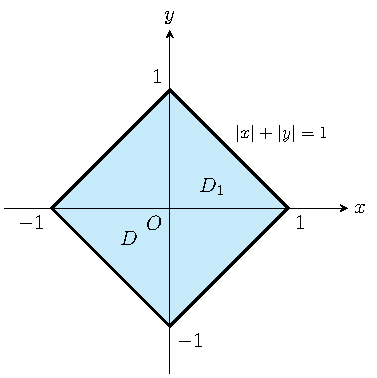
\includegraphics[width=\linewidth]{2018x-figure1.pdf} % 引入图片源
      \end{minipage}

    \item \textbf{Solution}.

      \noindent
      \begin{minipage}[c]{0.62\textwidth}
        设
        \[
          A=\iint\limits_{D}f(x,y)\,\mathrm{d}x\,\mathrm{d}y,
        \]

        则$f(x,y)=xy+A$.

        于是
        \[
          \begin{aligned}
            A & =\iint\limits_{D}xy\,\mathrm{d}x\,\mathrm{d}y+\iint\limits_{D}A\,\mathrm{d}x\,\mathrm{d}y                          \\
              & =\int_{0}^{1}\,\mathrm{d}x\int_{0}^{x^{2}}xy\,\mathrm{d}y +A\int_{0}^{1}\,\mathrm{d}x\int_{0}^{x^{2}}\,\mathrm{d}y \\
              & =\frac{1}{12}+\frac{A}{3}.
          \end{aligned}
        \]

        解得$A=\frac{1}{8}$，故
        \[
          f(x,y)=xy+\frac{1}{8}.
        \]
      \end{minipage}
      \hfill %
      \begin{minipage}[c]{0.28\textwidth}
        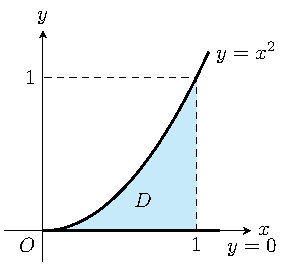
\includegraphics[width=\linewidth]{2018x-figure2.pdf} % 引入图片源
      \end{minipage}

    \item \textbf{Solution}. 旋转曲面方程为
      \[
        z=\frac{1}{2}(x^{2}+y^{2}).
      \]

      记$\Omega$在$xOy$面上的投影区域为$D:x^{2}+y^{2}\leq16$. 用柱坐标代换，得
      \[
        \begin{aligned}
          I & =\iiint\limits_{\Omega}(x^{2}+y^{2})\,\mathrm{d}v                                                      \\
            & =\int_{0}^{2\pi}\,\mathrm{d}\theta\int_{0}^{4}r\,\mathrm{d}r \int_{\frac{1}{2}r^{2}}^{8}r^{2}\,\mathrm{d}z \\
            & =2\pi\int_{0}^{4}r^{3}\left(8-\frac{r^{2}}{2}\right)\,\mathrm{d}r =\frac{1024\pi}{3}.
        \end{aligned}
      \]

    \item \textbf{Solution}. 由题设可知$\Omega$为上半球$x^{2}+y^{2}+z^{2}\leq a^{2}
      ,z\geq0$. 先对$z$积分，得
      \[
        \begin{aligned}
          I & =\int_{0}^{a}z^{2}\,\mathrm{d}z \iint\limits_{x^{2}+y^{2}\leq a^{2}-z^{2}}\,\mathrm{d}x\,\mathrm{d}y \\
            & =\pi\int_{0}^{a}z^{2}(a^{2}-z^{2})\,\mathrm{d}z =\frac{2\pi a^{5}}{15}.
        \end{aligned}
      \]
  \end{enumerate}

  \section{综合题(每小题 8 分，共 40 分)}
  \begin{enumerate}
    \setcounter{enumi}{10}

    \item \textbf{Solution}. 因为$\boldsymbol{n}=(3,4)$，所以其单位方向向量为$\boldsymbol
      {n}^{\circ}=\frac{1}{5}(3,4)$.

      又
      \[
        u_{x}=f'(x\sin y)\sin y,\qquad u_{y}=f'(x\sin y)x\cos y,
      \]
      所以
      \[
        \frac{\partial u}{\partial \boldsymbol{n}}=\frac{f'(x\sin y)}{5}(3\sin y+
        4x\cos y).
      \]

      利用偏导数定义，得
      \[
        \left.\frac{\partial^{2}u}{\partial \boldsymbol{n}\partial x}\right|_{(0,0)}
        =\lim_{x\to0}\frac{\dfrac{\partial u}{\partial \boldsymbol{n}}(x,0) -\dfrac{\partial u}{\partial \boldsymbol{n}}(0,0)}{x}
        =\lim_{x\to0}\frac{\frac{4}{5}f'(0)x}{x}=4.
      \]

    \item \textbf{Solution}. 设所求点为$M(x,y)$，则$\nabla f(x,y)=(6x,2y)$，且$\boldsymbol
      {n}^{\circ}=\frac{1}{5}(3,4)$.

      函数$f(x,y)$在点$M(x,y)$沿方向$\boldsymbol{n}$的方向导数为
      \[
        \frac{\partial f}{\partial \boldsymbol{n}}(x,y)=\frac{1}{5}(18x+8y) =\frac{2}{5}
        (9x+4y).
      \]

      因此在约束$x^{2}+2y^{2}-2x=88$下求$9x+4y$的最大值. 构造Lagrange函数
      \[
        L(x,y,\lambda)=9x+4y+\lambda(x^{2}+2y^{2}-2x-88).
      \]

      令
      \[
        \begin{cases}
          L_{x}=9+2\lambda x-2\lambda=0,    \\
          L_{y}=4+4\lambda y=0,             \\
          L_{\lambda}=x^{2}+2y^{2}-2x-88=0.
        \end{cases}
      \]

      由前两个方程可得$2(x-1)=9y$，代入约束方程得两个受检点
      \[
        M_{1}(10,2),\qquad M_{2}(-8,-2).
      \]

      比较方向导数的值，得$M_{1}(10,2)$为所求点.

    \item \textbf{Solution}.

      \noindent
      \begin{minipage}[c]{0.57\textwidth}
        区域$D$由抛物线$y^{2}=ax$和圆$x^{2}+y^{2}=2ax$围成，联立
        \[
          \begin{cases}
            y^{2}=ax,       \\
            y^{2}=2ax-x^{2}
          \end{cases}
        \]
        得交点$(0,0),(a,a),(a,-a)$.

        所求面积为
        \[
          \begin{aligned}
            S & =\frac{1}{2}\pi a^{2}+2\int_{0}^{a}\,\mathrm{d}y\int_{\frac{y^{2}}{a}}^{a}\,\mathrm{d}x                                  \\
              & =\frac{1}{2}\pi a^{2}+2\int_{0}^{a}\left(a-\frac{y^{2}}{a}\right)\,\mathrm{d}y =\frac{1}{2}\pi a^{2}+\frac{4}{3}a^{2}.
          \end{aligned}
        \]
      \end{minipage}
      \hfill %
      \begin{minipage}[c]{0.33\textwidth}
        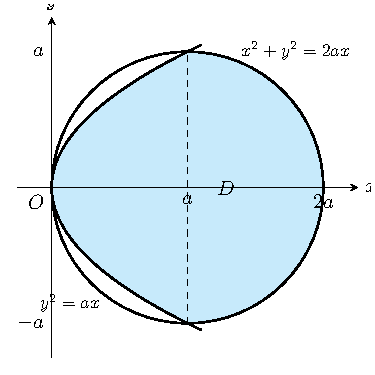
\includegraphics[width=\linewidth]{2018x-figure3.pdf} % 引入图片源
      \end{minipage}

    \item \textbf{Solution}.

      \noindent
      \begin{minipage}[c]{0.57\textwidth}
        记$D_{1}:x^{2}+y^{2}\leq1$，$D_{2}=D\setminus D_{1}$，并设$g(x,y)=x^{2}+y
        ^{2}-1$.

        则
        \[
          \begin{aligned}
            I= & -\iint\limits_{D_{1}}g(x,y)\,\mathrm{d}x\,\mathrm{d}y+\iint\limits_{D_{2}}g(x,y)\,\mathrm{d}x\,\mathrm{d}y \\
            =  & \iint\limits_{D}g(x,y)\,\mathrm{d}x\,\mathrm{d}y-2\iint\limits_{D_{1}}g(x,y)\,\mathrm{d}x\,\mathrm{d}y.
          \end{aligned}
        \]

        而
        \[
          \iint\limits_{D}g(x,y)\,\mathrm{d}x\,\mathrm{d}y =\int_{-2}^{2}\int_{-2}^{2}
          (x^{2}+y^{2}-1)\,\mathrm{d}y\,\mathrm{d}x =\frac{80}{3},
        \]
        且
        \[
          \iint\limits_{D_{1}}g(x,y)\,\mathrm{d}x\,\mathrm{d}y =\int_{0}^{2\pi}\,\mathrm{d}
          \theta\int_{0}^{1}(r^{2}-1)r\,\mathrm{d}r =-\frac{\pi}{2}.
        \]

        所以
        \[
          I=\frac{80}{3}+\pi.
        \]
      \end{minipage}
      \hfill %
      \begin{minipage}[c]{0.33\textwidth}
        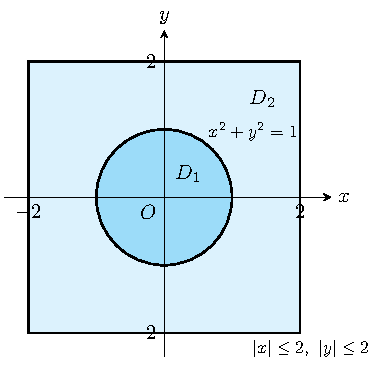
\includegraphics[width=\linewidth]{2018x-figure4.pdf} % 引入图片源
      \end{minipage}

    \item \textbf{Solution}.

      （1）正确. 因为根据偏导数定义，
      \[
        f_{xx}(0,0)=\left.\frac{\mathrm{d}f_{x}(x,0)}{\mathrm{d}x}\right|_{x=0},
      \]
      而一元函数可导必连续，所以$f_{x}(x,0)$在$x=0$处连续.

      （2）不正确. 例如
      \[
        f(x,y)=
        \begin{cases}
          0, & xy=0,    \\
          1, & xy\neq0.
        \end{cases}
      \]

      该函数在原点$(0,0)$处不连续. 但是因为$f(x,0)=0$，所以$f_{x}(x,0)=0$，进而$f
      _{xx}(0,0)=0$；

      类似可得$f_{yy}(0,0)=0$. 因此即使$f_{xx}(0,0)$和$f_{yy}(0,0)$存在，$f(x,y)$也未必在原点连续.
  \end{enumerate}
\end{document}






